% Notas breves de Belinda Toaquiza. Compilar notas/main.tex.
\section*{\personaUno{} · RPC}
\textbf{Proyecto:} SGRA gestiona solicitudes de refuerzo entre estudiantes y docentes. \textbf{Alcance:} revisión de código y propuesta futura.

\subsection*{Teoría y ejemplo}
Explicaré RPC como una llamada a una operación de otro proceso: el contrato define método y datos, el \emph{stub} representa al servicio y la serialización prepara los mensajes. El servidor ejecuta la operación y devuelve el resultado; siguen existiendo latencia y posibles fallos \cite{zhang2023rpc,arcuri2025evomaster}.

Demostraré \texttt{consultarDocenteAsignado} con JSON-RPC sobre HTTP: \texttt{servidor.py} permanece activo en una terminal y \texttt{cliente.py 101 12} solicita el docente en otra. La respuesta devuelve ID 7 y conserva el \texttt{id} de llamada. Con \texttt{101 99}, responde \emph{sin asignación}, distinto de una desconexión. \texttt{ejecutar.ps1} facilita el arranque. La demo no consulta PostgreSQL ni autentica usuarios.

\subsection*{Propuesta y decisiones}
Actualmente, Angular consulta al backend por HTTP y la creación de solicitudes usa una llamada Java interna para obtener el docente. Propondré extraer esa consulta a un servicio académico, con modelo cliente--servidor y petición--respuesta síncrona mediante JSON-RPC sobre HTTPS, conservando la identidad autenticada y una base PostgreSQL sin réplicas ni caché. El bosquejo y el TikZ distinguen ese cambio del estado actual.

Ofreceríamos transparencia de ubicación, manteniendo la API de Angular; la de fallos sería limitada. Un corte impide verificar el docente y detiene ese flujo de alta. Esto no demuestra una etiqueta CP. Con red sana leeríamos la fuente primaria y mediríamos p50/p95 y errores; sin definir replicación y garantías no asignaríamos PC/EC \cite{ahmed2023consistency}.

\subsection*{Fallo, comparación y conclusión}
El fallo \textbf{supuesto} es un reinicio del servicio durante la consulta. El timeout requiere registros para confirmar su causa. Recuperado el servicio, repetiríamos solo la lectura, no el alta completa. La prueba del cliente con servidor detenido no valida el comportamiento integrado de SGRA.

Moodle con Scheduler organiza citas docente--estudiante dentro de Moodle \cite{moodle2025scheduler}; SGRA gestiona solicitudes de refuerzo y propone separar la consulta: permite reutilizarla, pero añade comunicación y operación. No se comparó rendimiento. Concluiré que debemos validar identidad, trazas, corte y recuperación antes de distribuir más funciones.

\textbf{Evidencias:} carpetas \path{Belinda T/} en demo, diagrama y evidencias; bosquejo del 19-11-2026 y capturas personales del 20-11-2026.

{\small\textbf{Lecturas revisadas:} Zhang (manuscrito, p.~3), Arcuri (p.~3) y Ahmed (p.~172); las capturas incluyen síntesis breves y declaran la asistencia de IA. Belinda confirmó su lectura.}

\begin{minipage}{\linewidth}
\textbf{Bosquejo inicial de la propuesta}\par\smallskip
\begin{minipage}[c]{.22\linewidth}
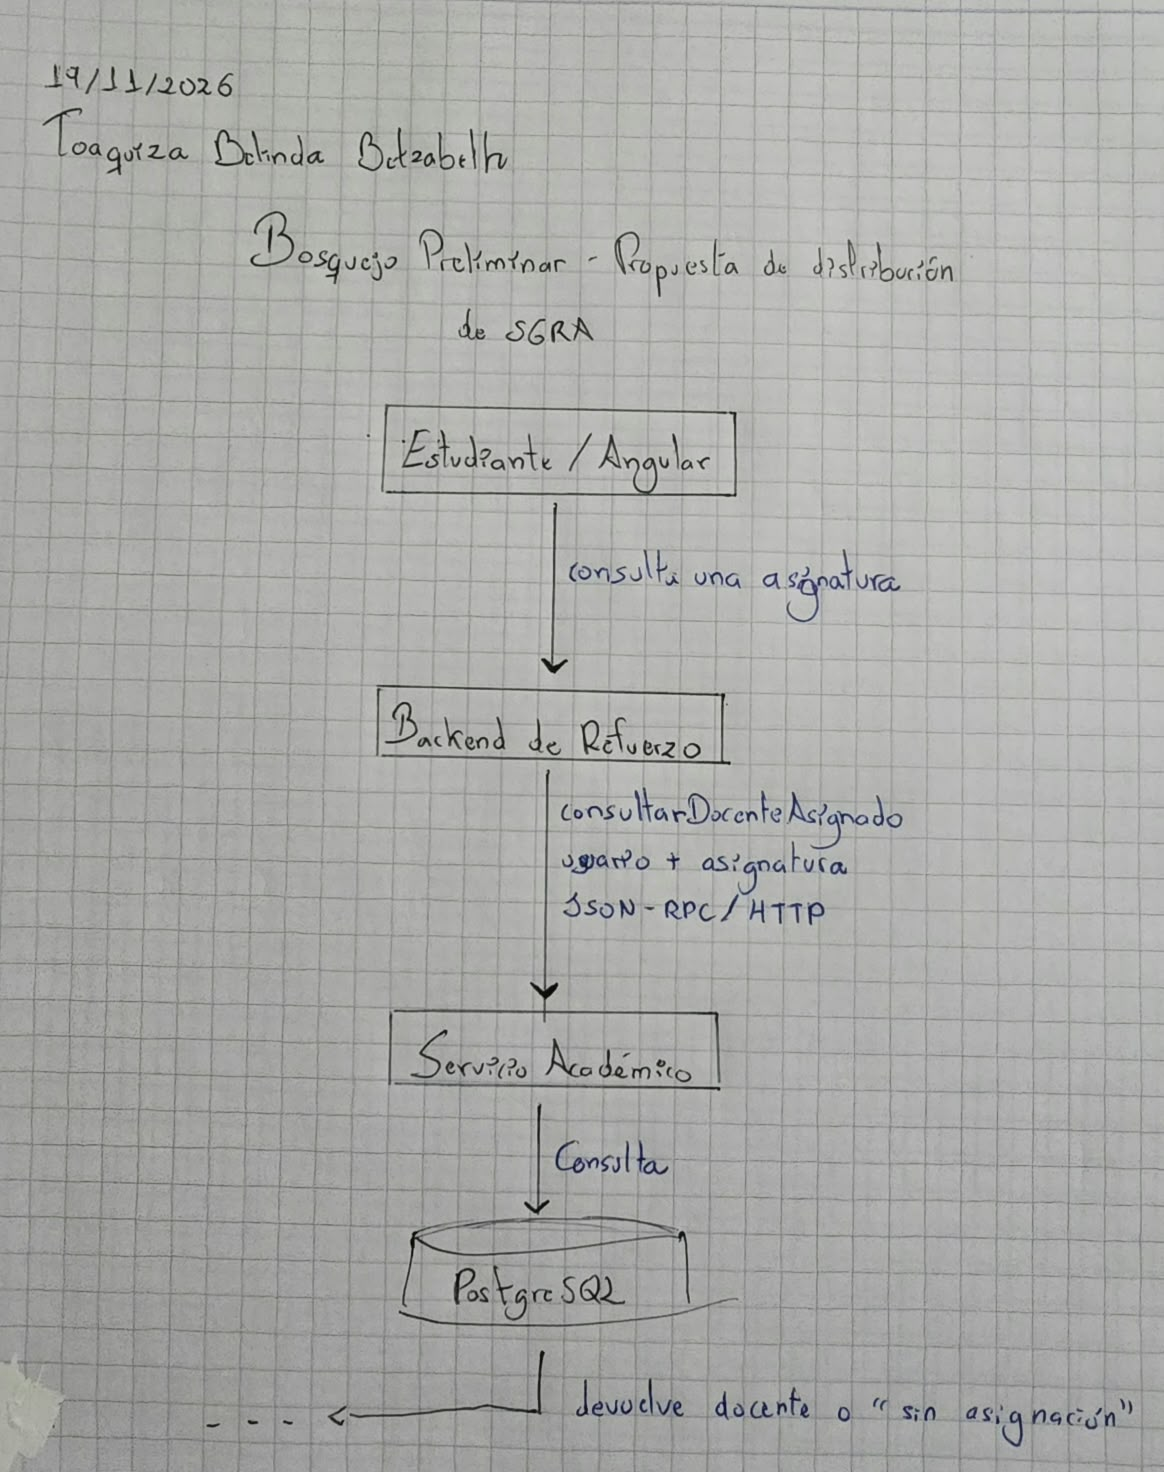
\includegraphics[height=.16\textheight,keepaspectratio]{../evidencias/Belinda T/esquema-mano/sgra-bosquejo-preliminar-consulta-docente-belinda-2026-11-19.jpeg}
\end{minipage}\hfill
\begin{minipage}[c]{.75\linewidth}
{\small Bosquejo manuscrito original de Belinda Toaquiza, 19-11-2026, con nombre y fecha visibles. Plantea el recorrido Angular, refuerzos, servicio académico y PostgreSQL. El TikZ posterior precisa los límites de proceso, la identidad y las respuestas. La fotografía completa está en \path{evidencias/Belinda T/esquema-mano/}.}
\end{minipage}
\end{minipage}
